
%% Web interface
\section{The Web Interface}

The purpose of the web interface is to grant a simpler way for users to interact with the interpreters.
This is split up into two parts:
The server, which handles the routing of the web server and serves the client interface along with API-calls for the actual interaction with the command-line interpreters, and the client part, which is the actual web interface that the user sees.
This chapter described the implementation of these.

\subsection{Client Interface}
\label{sec:implementation_web_client}

%%%%%%%%%%%%%%%%%%%
%%% Features
%%%%%%%%%%%%%%%%%%%

\subsubsection{Features}

Before explaining the actual implementation of the client interface, we will describe the features of this interface.
If we look at the user interface (seen in Appendix~\ref{fig:web_client_ui}), we have 3 rectangular areas: The toolbar at the top, the code editor located below the toolbar on the left-hand side, and the result area located below the toolbar on the right-hand side.

%\begin{figure}
%  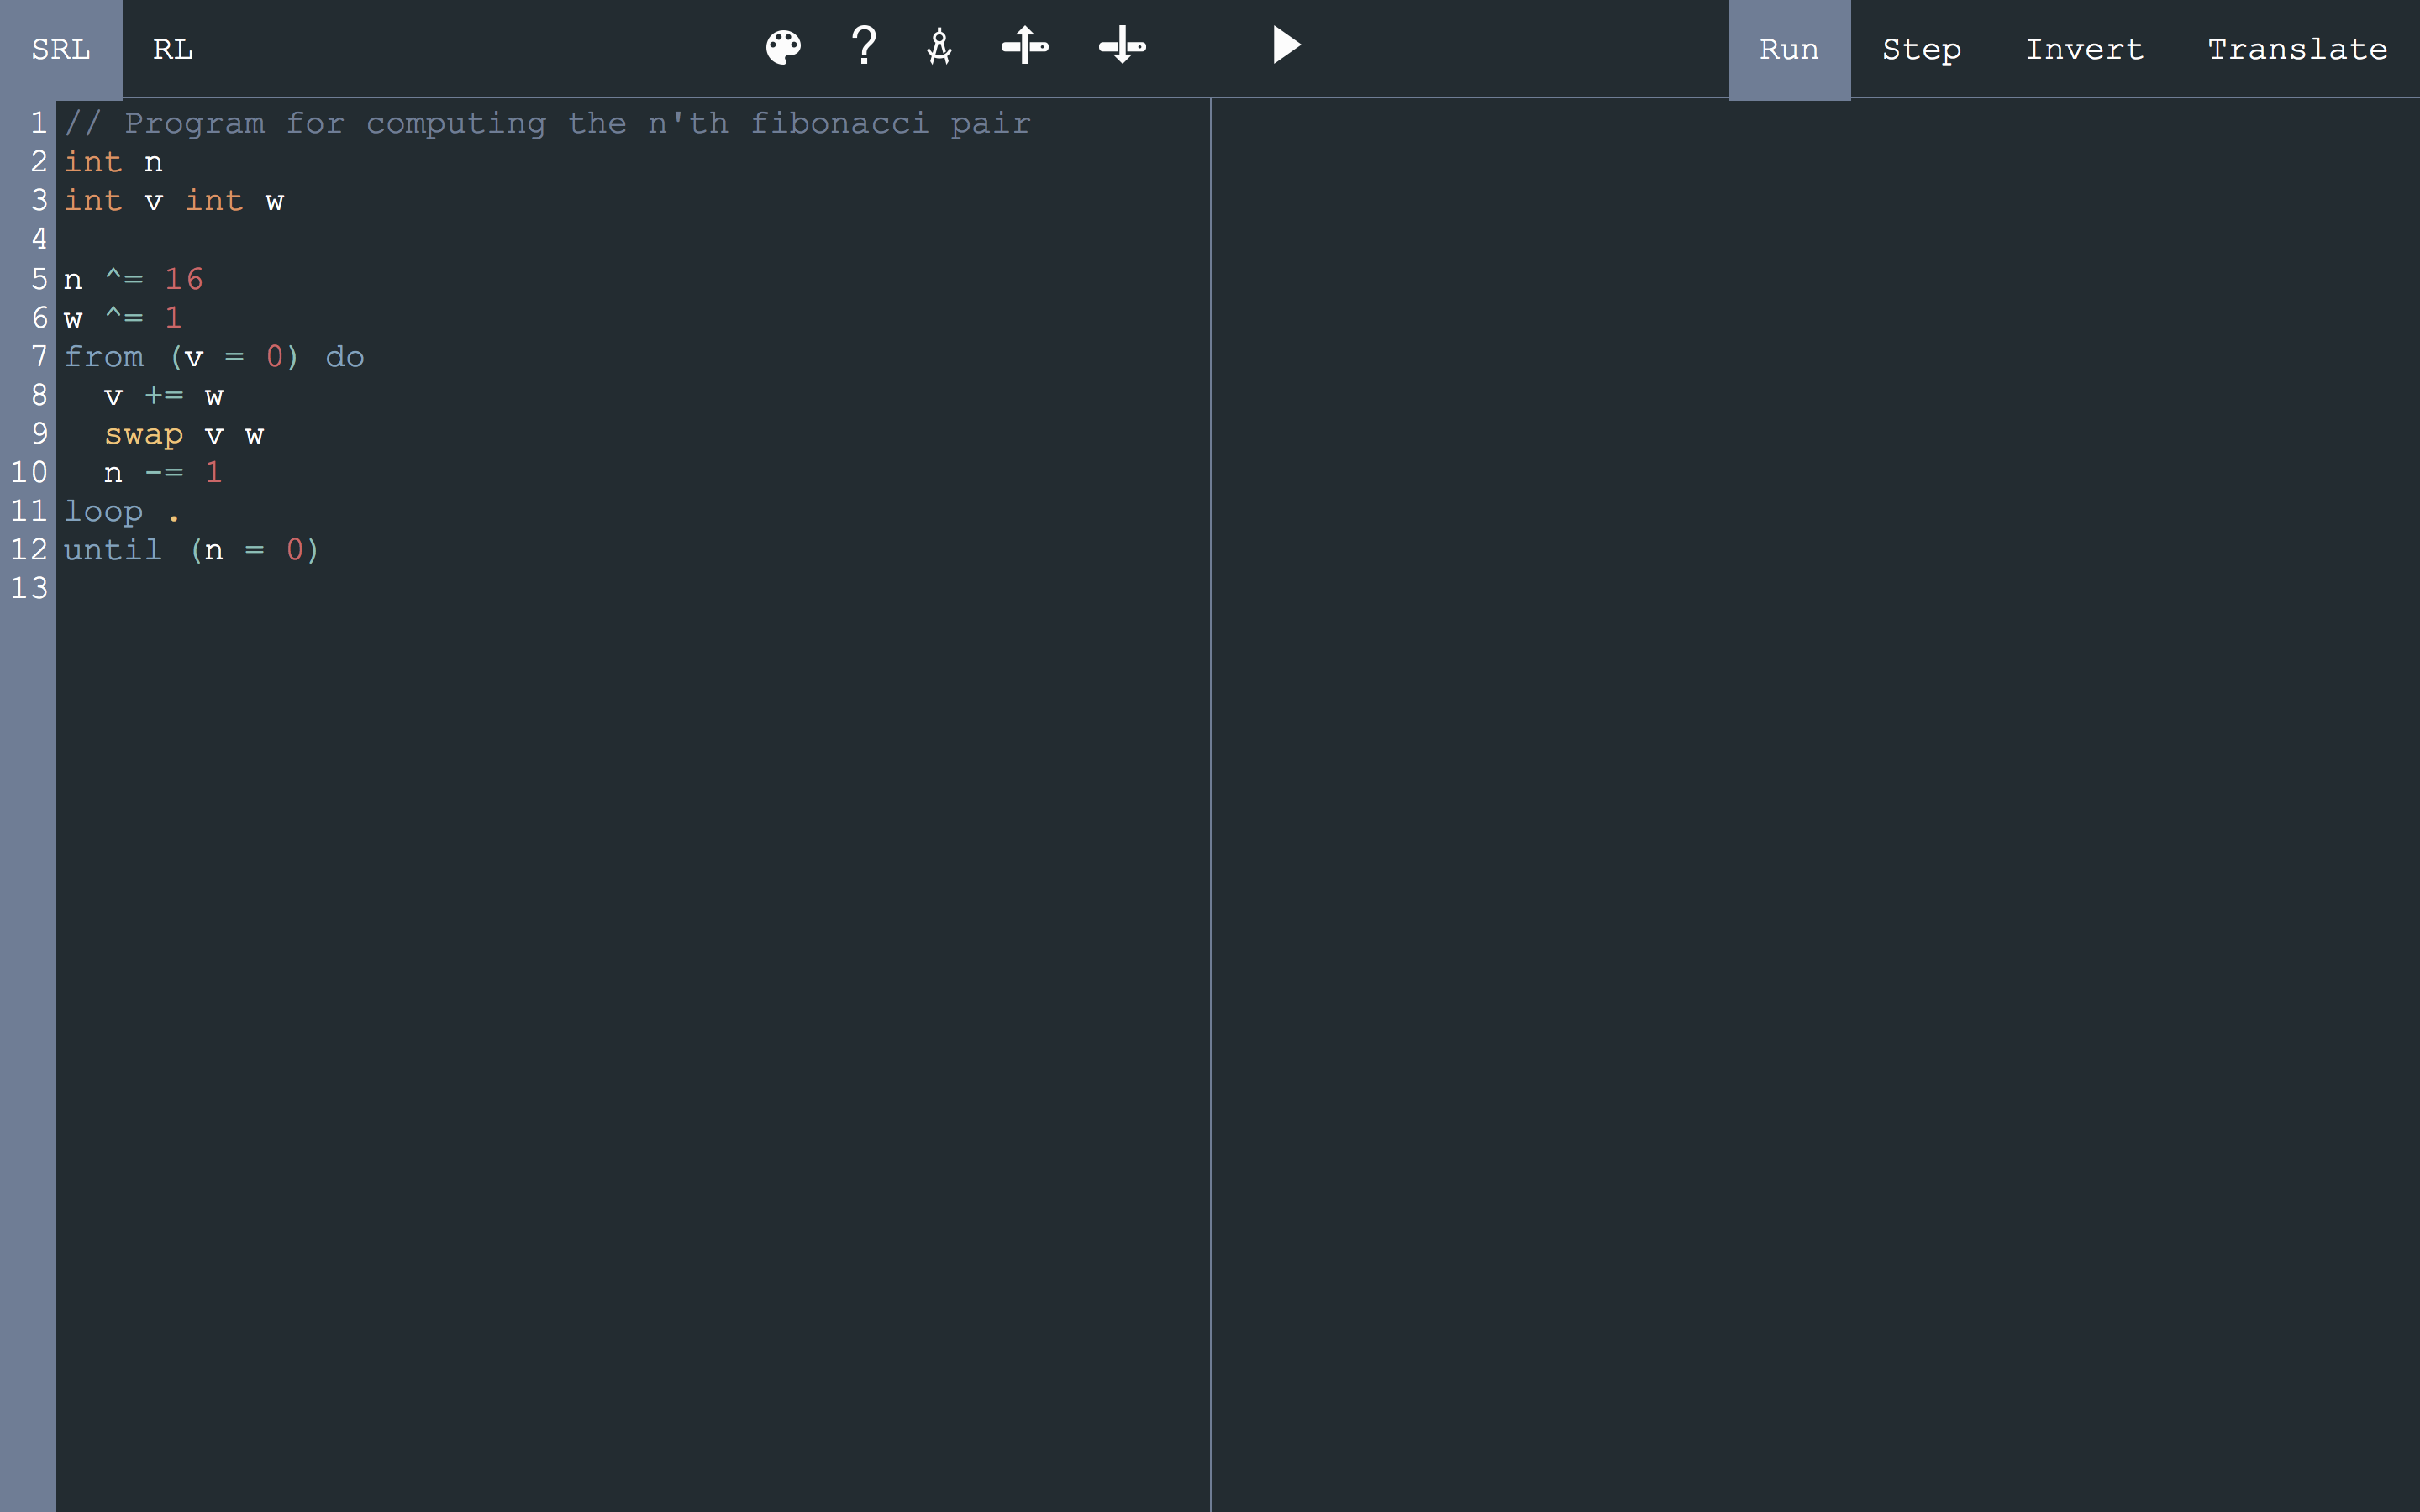
\includegraphics[width=\textwidth]{web_client_ui.png}
%  \caption{Screenshot of web client UI.}
%  \label{fig:web_client_ui}
%\end{figure}

At the far left of the toolbar we have two radio buttons with the options SRL and RL, respectively. The highlighted option indicates how the code in the code editor should be interpreted; if RL is chosen, the code is interpreted as an RL program and similarly, if SRL is chosen, the code is interpreted as an SRL program.

In the middle of the toolbar, above the code editor, we have a group of five icons:
\begin{description}

  \item[\inlineicon{themes.png} Themes]~\\
    By hovering over this icon a dropdown menu, for choosing the color scheme/ theme of the client interface, appears. %This can be seen in Fig.~\ref{app:web_client_themes}.
    %Fig. \ref{fig:web_client_white_ui} shows the color scheme when the white theme is chosen.
    %\begin{figure}
    %  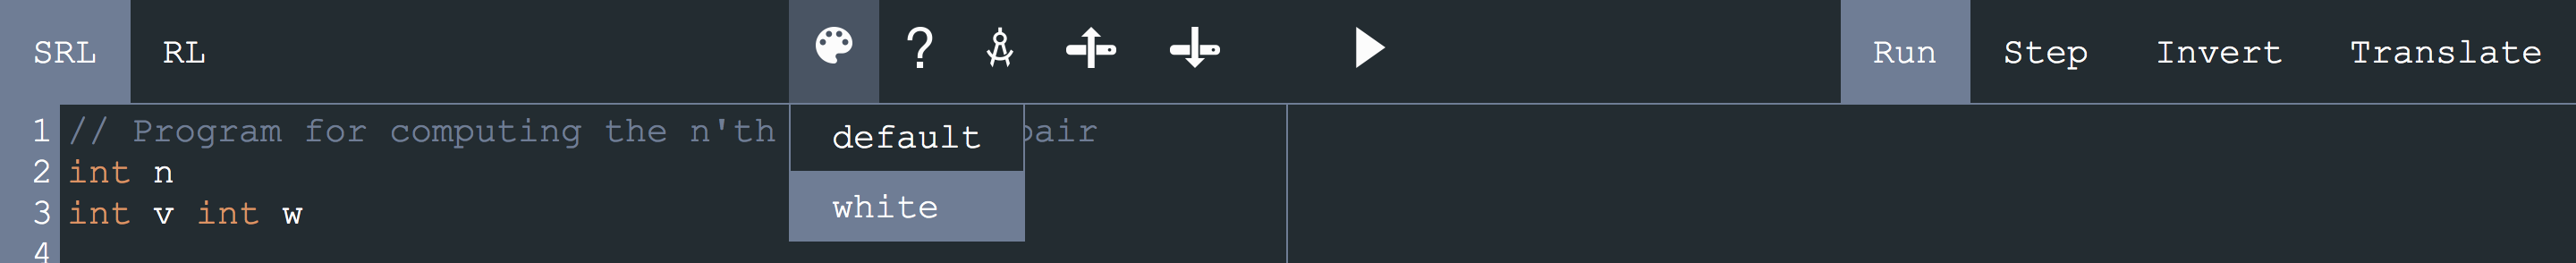
\includegraphics[width=\textwidth]{web_client_themes.png}
    %  \caption{Web client themes dropdown menu.}
    %  \label{fig:web_client_themes}
    %\end{figure}
    %\begin{figure}
    %  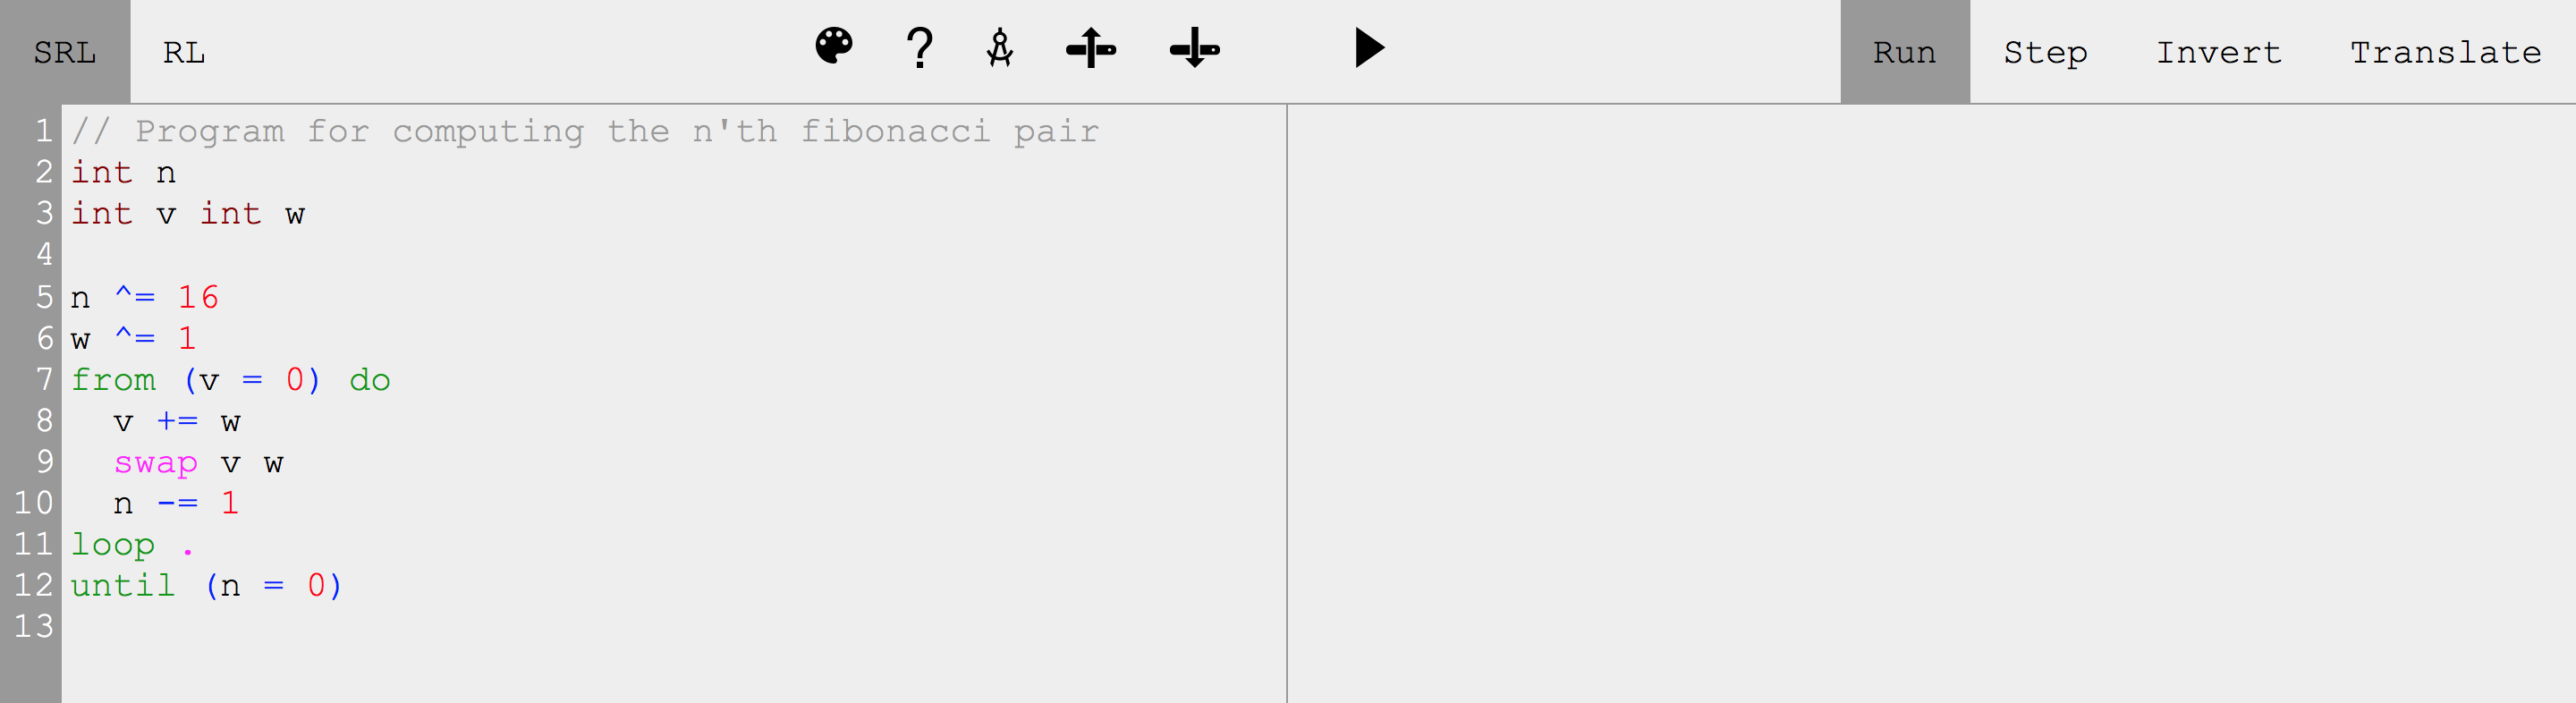
\includegraphics[width=\textwidth]{web_client_white_ui.png}
    %  \caption{Web client UI in white theme color scheme.}
    %  \label{fig:web_client_white_ui}
    %\end{figure}

  \item[\inlineicon{help.png} Help]~\\
    By clicking on this icon a modal window displaying some help text opens. This help text seeks to explain the web interface, the modes and the languages to the user.
    %\begin{figure}
    %  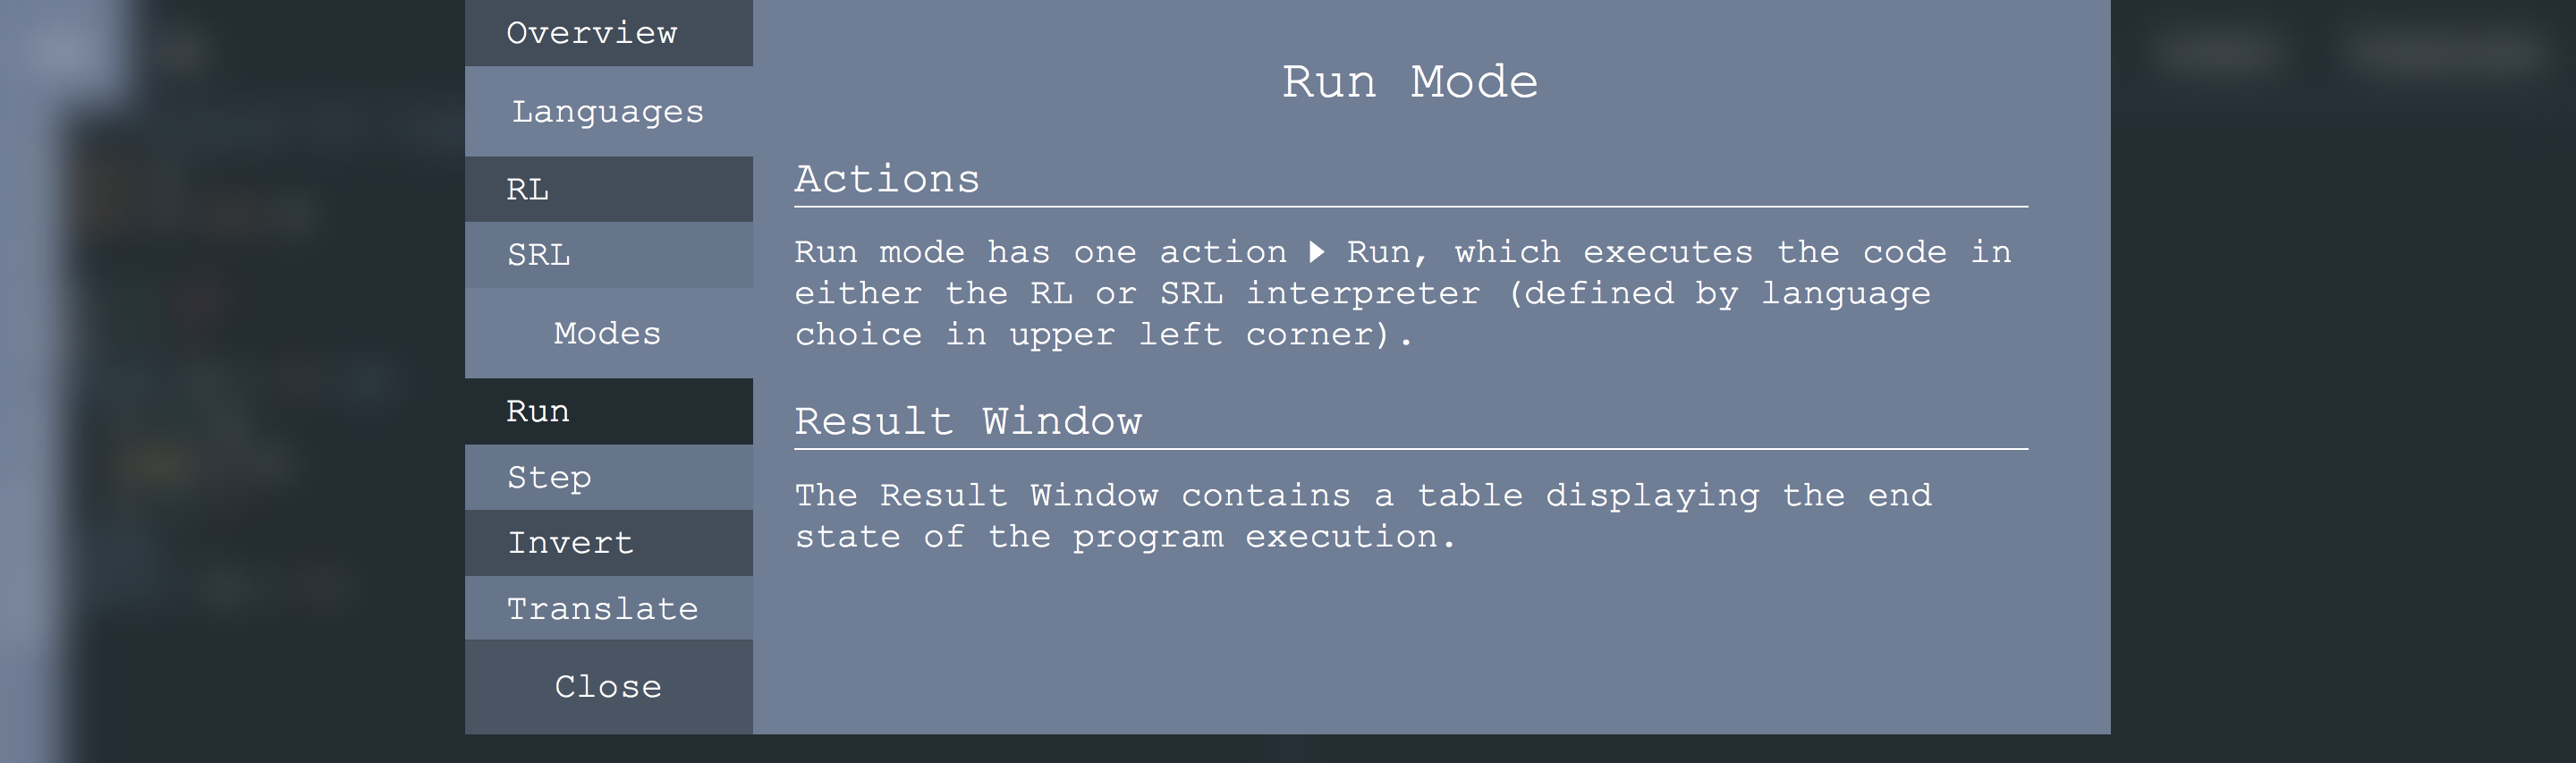
\includegraphics[width=\textwidth]{web_client_help.png}
    %  \caption{Web client help modal window displaying the Run mode help page.}
    %  \label{fig:web_client_help}
    %\end{figure}

  \item[\inlineicon{template.png} Templates]~\\
    By hovering over this icon a dropdown menu appears. This menu contains a series of template programs for both RL and SRL which can be loaded into the code editor.
    %\begin{figure}
    %  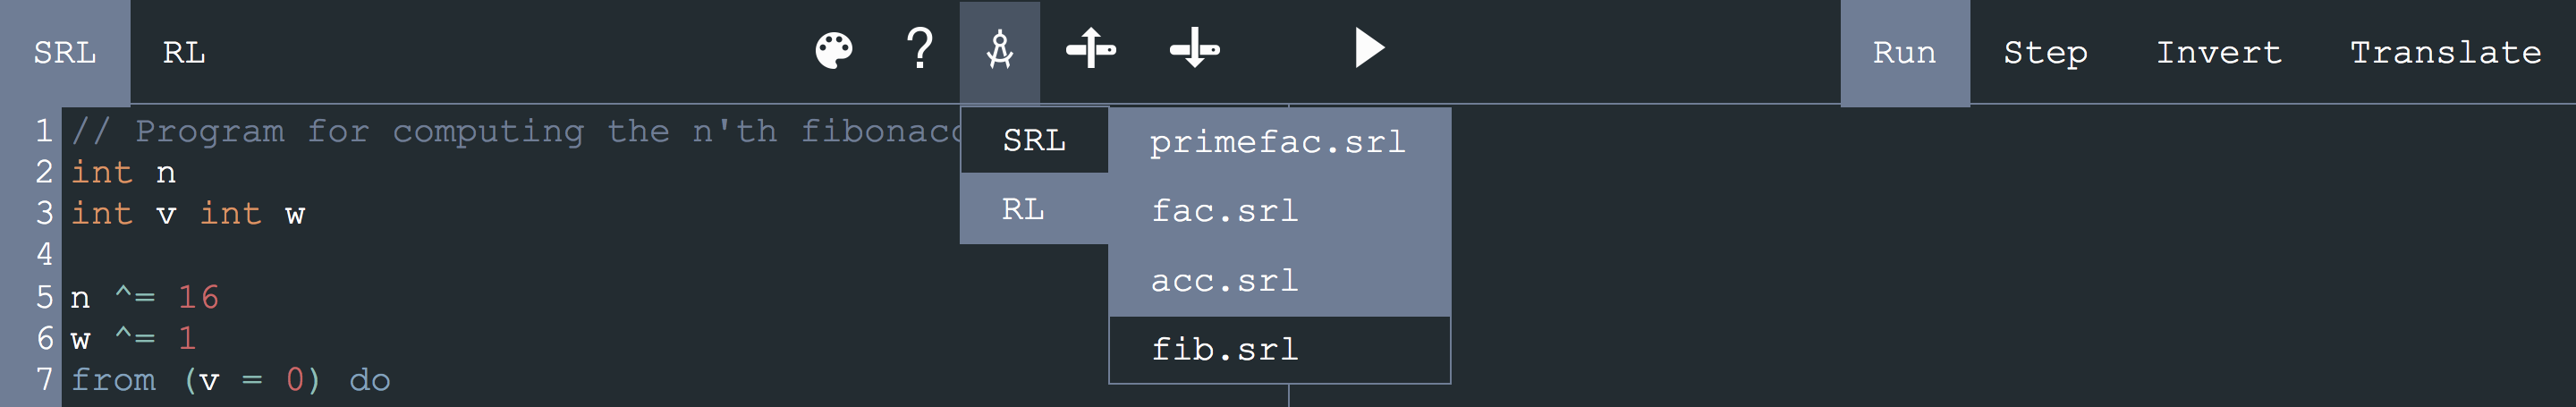
\includegraphics[width=\textwidth]{web_client_templates.png}
    %  \caption{Web client templates dropdown menu.}
    %  \label{fig:web_client_templates}
    %\end{figure}

  \item[\inlineicon{open.png} Open]~\\
    By clicking on this icon a modal window opens. Here it is possible to import and open previously stored programs.
    %\begin{figure}
    %  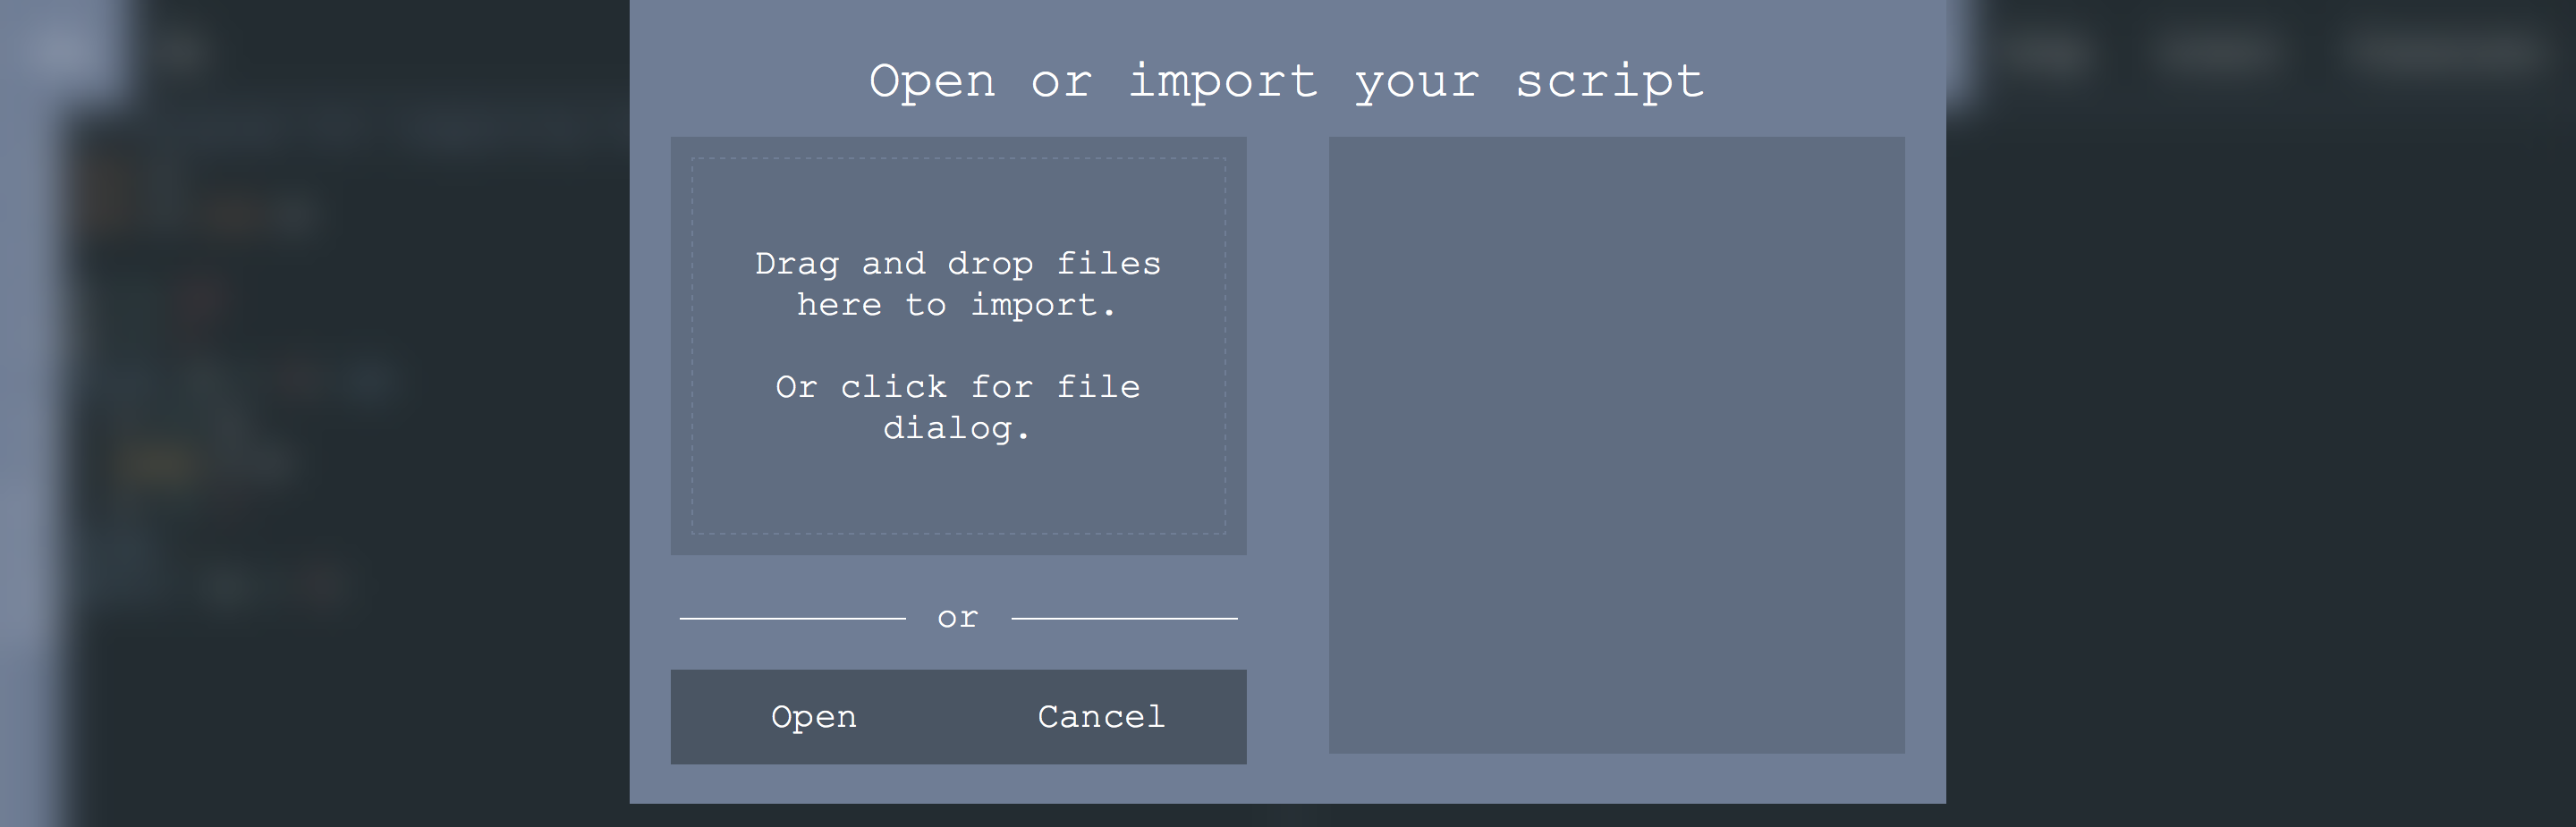
\includegraphics[width=\textwidth]{web_client_open.png}
    %  \caption{Web client open modal window.}
    %  \label{fig:web_client_open}
    %\end{figure}

  \item[\inlineicon{save.png} Save]~\\
    By clicking on this icon a modal window opens. Here it is possible to export, share and store the code currently loaded into the code editor.
    %\begin{figure}
    %  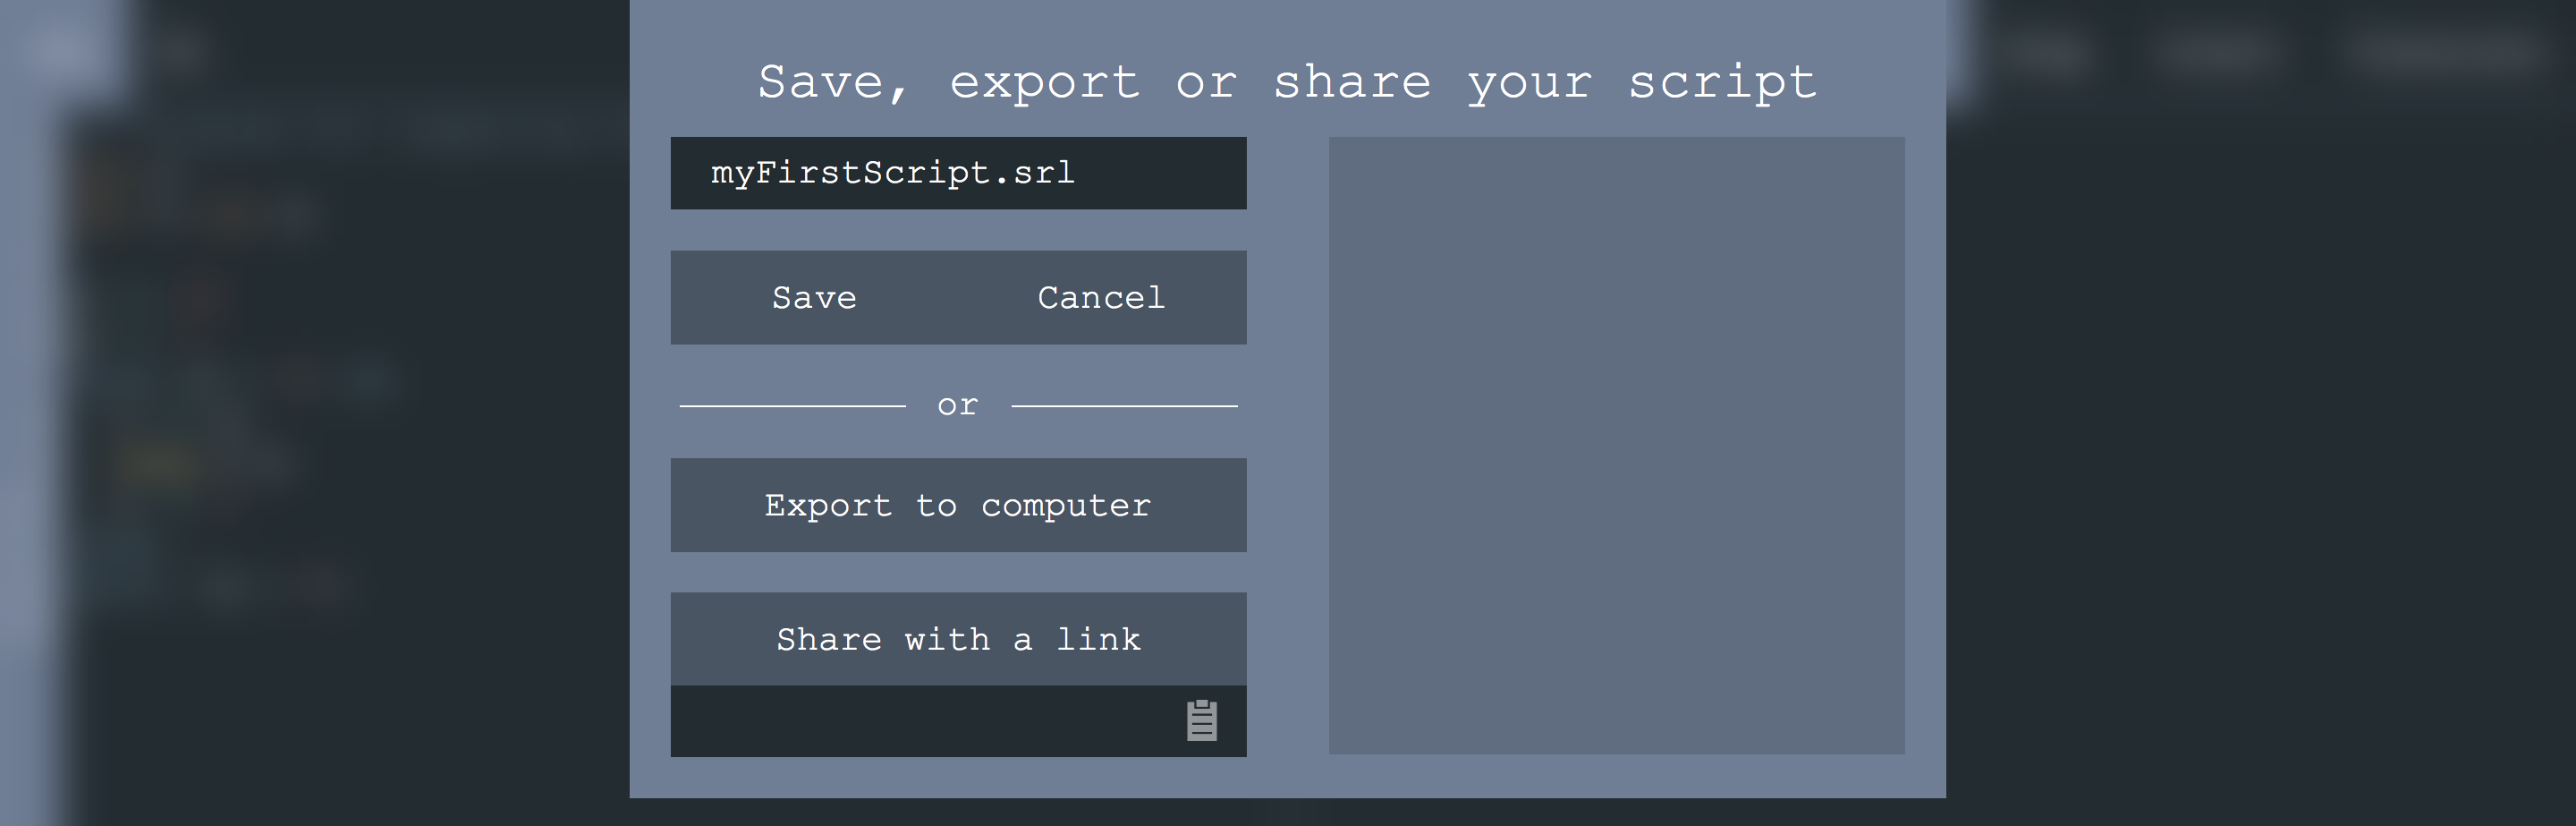
\includegraphics[width=\textwidth]{web_client_save.png}
    %  \caption{Web client save modal window.}
    %  \label{fig:web_client_save}
    %\end{figure}

\end{description}
The right-hand side of the toolbar is dedicated to modes and their associated actions.

There are 4 modes which are selected from the radio button group at the far right:
\begin{description}

  \item[Run]~\\
    The \textit{Run} mode simply executes the code in the editor depending on the chosen language. This is done by clicking \inlineicon{play} \textbf{run}.

  \item[Step]~\\
    The \textit{Step} mode allows for step-by-step program execution. %This even makes for a simple debugger.
    To begin the step-by-step execution, one has to click on \inlineicon{play} \textbf{begin stepping}. Then, the user has five options:
    \inlineicon{prev} \textbf{previous step} undoes the last executed step operation;
    \inlineicon{next} \textbf{next step} executes the next step operation;
    \inlineicon{reset} \textbf{reset} undoes all executed step operations;
    \inlineicon{exec} \textbf{end} executes all remaining step operations;
    \inlineicon{stop} \textbf{stop} stops the execution and leaves the step-by-step execution.
    While in step-by-step execution, all other features are disabled.

  \item[Invert]~\\
    The \textit{Invert} mode simply inverts the code in the editor depending on the chosen language. This is done by clicking \inlineicon{play} \textbf{invert}.

  \item[Translate]~\\
    The \textit{Translate} mode translates the code in the editor depending on the chosen language. This is done by clicking \inlineicon{play} \textbf{translate}.

\end{description}
All the above modes have the ability to fail on a parse- or static error. % Fig. \ref{fig:web_client_error} illustrates a case where a parse error occurs.

%\begin{figure}
%  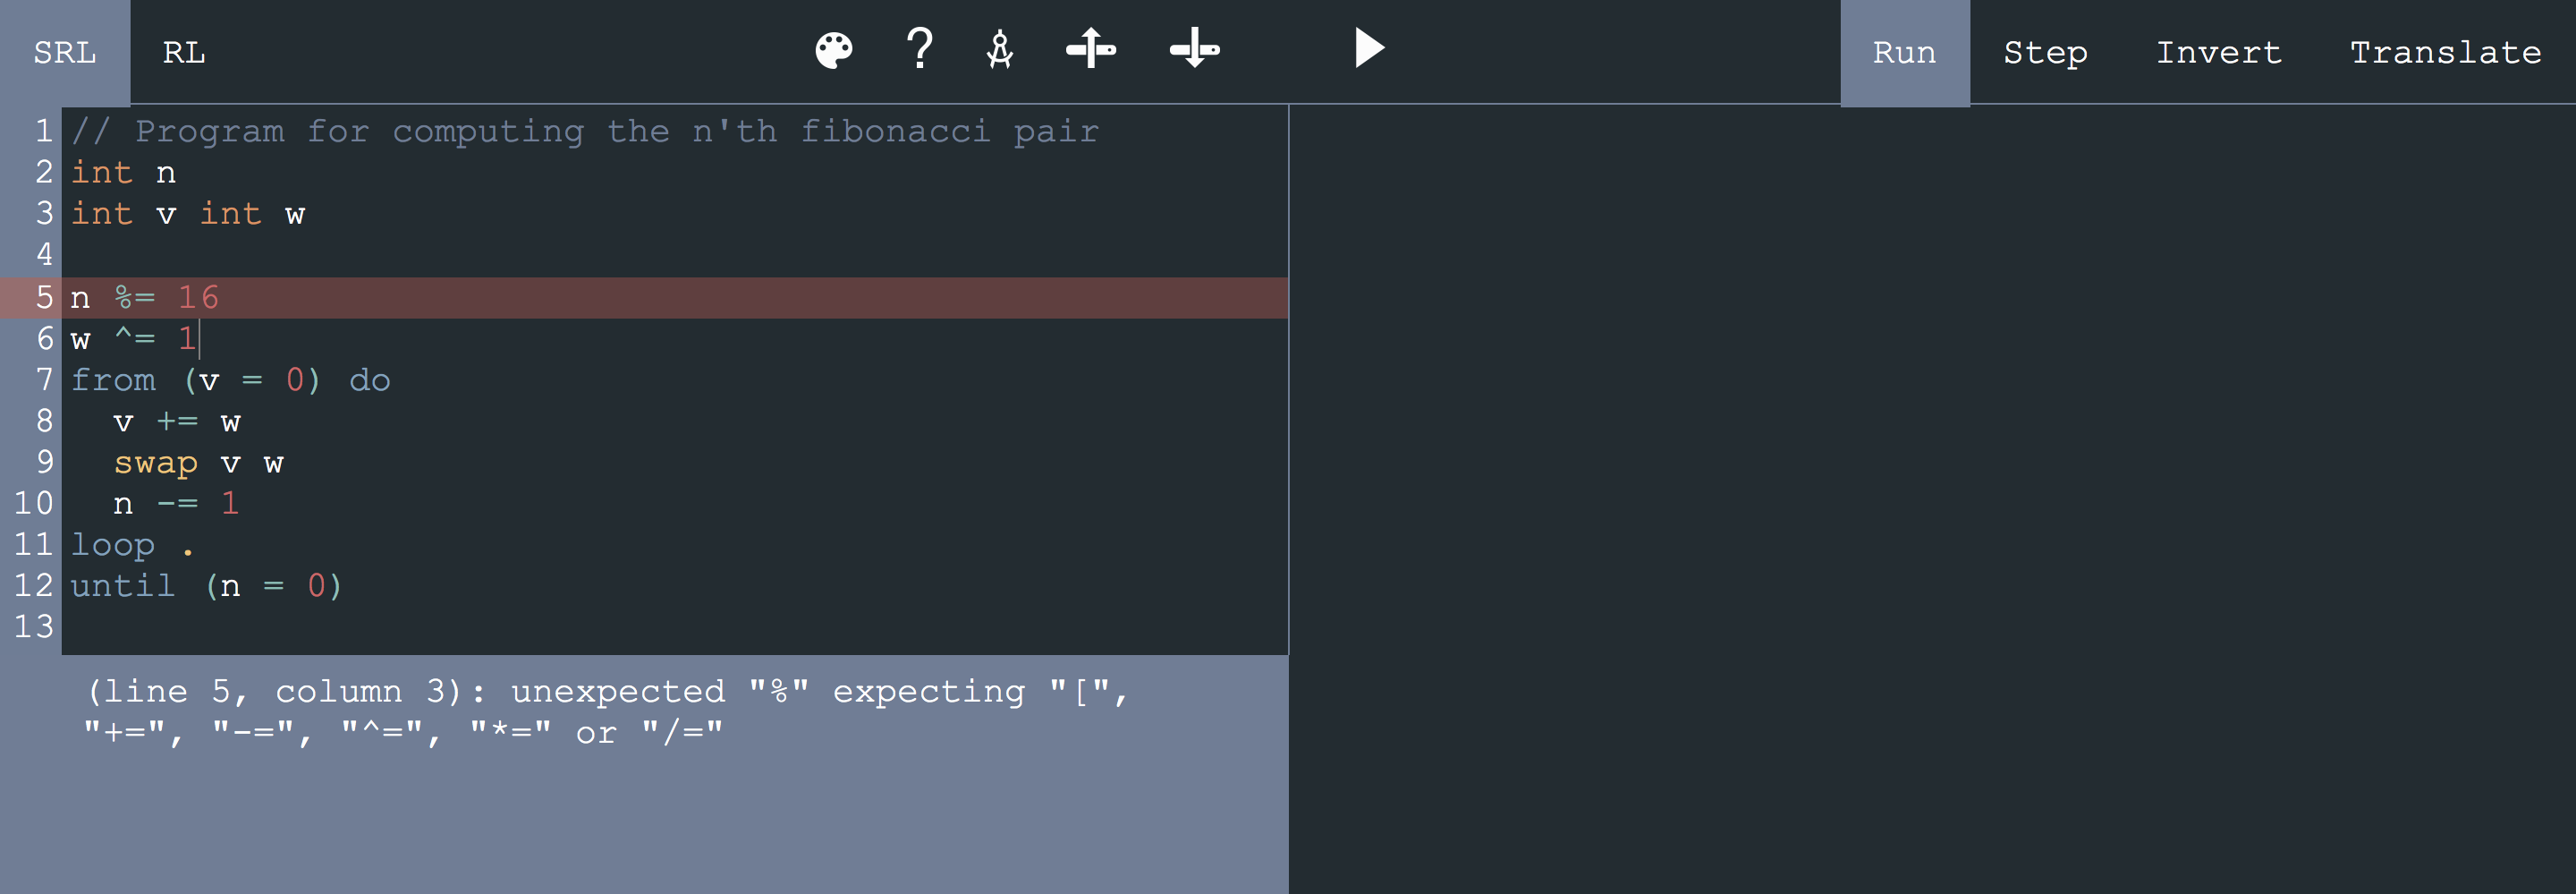
\includegraphics[width=\textwidth]{web_client_error.png}
%  \caption{Web client with parse error.}
%  \label{fig:web_client_error}
%\end{figure}

%%%%%%%%%%%%%%%%%%%
%%% Implementation
%%%%%%%%%%%%%%%%%%%

\subsubsection{Implementation}

Now that the features have been introduced, we can briefly look at the implementation.
The web client interface is a nodeJS project written in ECMAScript 6, using the library ReactJS, for creating modularised components.
We chose to use ReactJS instead of vanilla javascript and html, since it allows component rendering based on state.
This way focus was primarily on state and logic instead of design and propagating state to the application.
To separate state and logic from UI even further, we chose to handle state through Redux.
This way we could move state and alteration of state outside of the ReactJS components, hereby giving the individual components access to only the absolute necessary state variables and state alterations methods. Thus, the possibilities of a specific state alteration failing are limited to the components with access which, in turn, makes it easier to debug and fix.

The web client interface uses babel and webpack to compile and bundle scripts and resources.
Webpack uses babel to convert JSX to React components and transpile ECMAScript 6 to ECMAScript 5 in order to allow for \texttt{import} statements.
Webpack itself is used to precompile SASS, which is used for styling, to CSS, appending prefixes to the CSS for better cross-browser support and bundling scripts, styles and assets for minimal HTTP requests.

The root of the web client is \path{/web/client}. Configuration files for node package dependencies and the webpack build flow are found here.
Under the subdirectory \path{src/} are all source files and resources located.
ReactJS components are found under \path{src/components} and the corresponding styling/ SASS files are found under \path{src/styles} along with the theme color schemes in the subdirectory \path{src/styles/themes}.

The root component is the \textit{App} component which contains all the major components as children.
The App component is wrapped in a redux provider which allows the app and all its children access to the application state and state modifiers.
The children components of the App component are:
\begin{description}

  \item[Header]~\\
    Utilises the Button, Radio and Dropdown components for letting the user interact with the application.

  \item[Editor]~\\
    The editor has two areas; the coding area, which is visible at all times, and the error area, which only is visible when an error is present.
    The code editor component is the javascript library CodeMirror \cite{CM} delivered through the react-wrapper React CodeMirror 2.
    CodeMirror was chosen since it has a library for lexing --- used for syntax highlighting --- along with a lot of customisation options and extendibility through plugin support.

  \item[Result]~\\
    The result area presents the the potential results of the actions associtated with a mode. A program state is displayed as a lists of values, a step log (under the Step mode --- is displayed as a list of individual step operations, and program transformations are displayed through a read-only CodeMirror instance.

  \item[Modals]~\\
    `Modals` covers the HelpModal, OpenModal and SaveModal components, which use the same Button, Radio and Dropwdown components as the Header.

\end{description}
For more information regarding the implementation, refer to the source code in Appendix \ref{app:web_client}.



\subsection{Server \& API}
\label{sec:server_and_api}

The web server is an independent node project which, when built, uses the client web interface and the command-line interfaces as dependencies.
These are built and copied into the web server project folder.
The command-line interface binaries are placed under \path{/web/server/bin} and the web client interface is placed under \path{/web/server/client}.

The server is written in ECMAScript 6, but since nodeJS (version 9 and below) does not support \texttt{import} statements natively, the Babel transpiler is used for running the ECMAScript 6 code as ECMAScript 5.
This is done in the entry-file \path{babel-server.js}, as a wrapper for the actual server configuration in \path{server.js}.
We run the transpiled code with node and use the Express package for opening ports, setting up the server and handling web-routes.
All communication between the API server and the client-side is formatted as JSON; as are the results from the command-line interfaces.
This way it is easy to parse data from the interpreter to the client interface via the API.

The server has Cross Origin Resource Sharing (CORS) enabled, to allow for separation of the API server and the client web interface.
This allows for the server to be hosted at one address, while the interface is hosted at another.
CORS is enabled by setting the appropriate headers. That is,
\lstinputlisting[language=javascript,firstline=10,firstnumber=10,lastline=15]{../web/server/server.js}
The routing has two responsibilities: to handle API calls, which can be seen in Fig. \ref{fig:full_api}, and to serve static files when the client interface is requested. The defined routes are listed in Fig. \ref{fig:server_routes}. Routes are divided into 3 categories: API routes, root requests and static files; where static files are the bundled css and javascript files that the client interface requires.
If the client interface is hosted at a different address than the API, the \path{/web/server/client} folder can be removed, causing the route for the index page and the static pages to respond with a 404 (page not found) status and page.
In this case, to get the client to point to the correct API address, change the API\_URL found variable in \path{/web/client/webpack.prod.config.js} and rebuild the client interface.

The API sub-URLs, along with their valid request method(s) and functionality, are described in Fig. \ref{fig:full_api}.
\begin{figure}
  \begin{tabular}{|l|l|p{6.7cm}|}\hline
    \textbf{Route} & \textbf{Method} & \textbf{Responsibility}\\\hline
    \texttt{/run/:language} & \texttt{POST} & Here \texttt{:language} can either be \texttt{rl} or \texttt{srl}.
                                                This API-call executes the code that is posted along with the request, and returns the end-state of the program.
                                                The code submitted should be wrapped in a JSON object, with the attribute \texttt{code}.\\\hline
    \texttt{/run/log/:language} & \texttt{POST} & Is equivalent to \texttt{/run/:language}, but instead of returning the end-state
                                                    alone, it also returns the json-formatted execution-log.\\\hline
    \texttt{/invert/:language} & \texttt{POST} & Here \texttt{:language} can either be \texttt{rl} or \texttt{srl}.
                                                This API-call inverts the code.
                                                The code submitted should be wrapped in a JSON object, with the attribute \texttt{code}.\\\hline
    \texttt{/translate/:language} & \texttt{POST} & Here \texttt{:language} can either be \texttt{rl} or \texttt{srl}.
                                                This API-call translates the code from the specified language to its counterpart.
                                                The code submitted should be wrapped in a JSON object, with the attribute \texttt{code}.\\\hline
    \texttt{/template/list}  & \texttt{GET} & Returns a list of SRL and RL files, as a JSON-object. The object has the attributes \texttt{srl} and \texttt{rl}, where each corresponding value is a list of template-names for that language. \\\hline
    \texttt{/template/:file} & \texttt{GET} & Here \texttt{:file} is the template requested.
                                              A JSON-object, with the attribute \texttt{code}, which contains the code of the requested template file, is returned.\\\hline
  \end{tabular}
  \caption{API routes.}
  \label{fig:full_api}
\end{figure}
\begin{figure}
  \begin{tabular}{|l|p{8.7cm}|}\hline
    \textbf{Route} & \textbf{Responsibility}\\\hline
    \texttt{/}     & Fetch the built client interface index page from \path{/web/server/client/index.html}.\\\hline
    \texttt{/api*} & Here \texttt{*} is everything after \texttt{/api}, which is forwarded to the API router. The API routes are described in Fig. \ref{fig:full_api}. \\\hline
    \texttt{/:filename.:ext}     & Here \texttt{:filename.:ext} matches a static resource, e.g. \texttt{bundle.js}. All static files are fetched from \path{/web/server/client}. Thus only files that the client interface uses can be requested.\\\hline
  \end{tabular}
  \caption{Routes for web server.}
  \label{fig:server_routes}
\end{figure}

For accessing the command-line interfaces and fetching template files, the interface \texttt{execFile(file, [arguments], callback)} from the node module child\_process is used.
\texttt{execFile} takes the arguments to the file as a list, where each element is treated as one argument.
Instead of opening a shell and calling the file, execFile executes the file directly, which disallows for injections such as '" \&\& ls \#' for getting information about the host system.

% \begin{lstlisting}[language=javascript]
% execFile(cmd,
%         [mode, code, flags],
%         {maxBuffer, timeout},
%         (err, stdout, stderr) => {
%   // ... callback content
% });
% \end{lstlisting}
